\chapter{Introducere}

\section{Context: IoT și casele inteligente}
În ultimii ani, conceptul de \textit{Internet of Things} (IoT) s-a mutat dintr-un termen de cercetare într-un fenomen care influențează direct modul în care folosim locuința. O „casă inteligentă” înseamnă, în practică, o rețea de senzori și actuatori conectați la o unitate de control care interpretează datele și execută acțiuni automate sau manuale, declanșate de utilizator. Studiul lui Alaa et al., un \textit{review} amplu al aplicațiilor Smart Home publicate până la momentul respectiv, propune o taxonomie a acestor aplicații pe domenii precum confortul rezidențial, securitatea, eficiența energetică și asistența pentru sănătate \cite{iot_smart_home_review}.

Adopția acestor tehnologii nu depinde doar de cât de avansat este hardware-ul, ci și de cât de mult au încredere utilizatorii în sistem. Marikyan et al. observă, pe baza unei meta-analize, că factorii decisivi sunt utilitatea percepută, ușurința de utilizare și îngrijorările legate de confidențialitate \cite{marikyan_smarthome_2019}. Acest lucru este relevant pentru tema lucrării de față, fiindcă explică de ce o platformă transparentă, care rulează local și pe care utilizatorul o poate inspecta, are sens chiar și atunci când există alternative comerciale.

Pe partea de comunicație, soluțiile actuale s-au mutat în mare parte de la modelul cerere-răspuns specific HTTP la o paradigmă asincronă bazată pe \textit{publish/subscribe}. Protocolul MQTT (Message Queuing Telemetry Transport) a devenit standardul \textit{de facto} pentru schimbul de mesaje între microcontrolere și server, în primul rând datorită overhead-ului redus și a faptului că un singur broker poate distribui eficient mesaje la mulți abonați \cite{mqtt_standard_iot}. În arhitectura HomeForge, MQTT joacă exact acest rol: este magistrala prin care firmware-ul ESP32 comunică cu backend-ul Django.

% FIGURĂ DE ADĂUGAT: o schemă conceptuală a unei case inteligente -
% senzori (DHT11, BMP180), actuatori (relee), un router/broker MQTT,
% serverul HomeForge și aplicația web. Sugestie: diagrama poate fi
% desenată în draw.io / Inkscape și salvată ca PDF în figuri/.
\begin{figure}[htbp]
    \centering
    % \includegraphics[width=0.85\textwidth]{figuri/conceptul_smart_home.pdf}
    \caption{Schema conceptuală a unei case inteligente integrate în HomeForge (figură de adăugat)}
    \label{fig:concept_smarthome}
\end{figure}

\section{Limitări ale soluțiilor comerciale}
Marea majoritate a produselor de pe piață (Google Nest, Amazon Alexa, Tuya, Sonoff și variațiunile lor) lucrează după un model centrat pe cloud: dispozitivul fizic trimite datele către serverele producătorului, acolo se rulează logica de automatizare și de acolo se trimit comenzile înapoi. Există trei probleme practice cu această abordare, observate sistematic în literatură \cite{vendor_lockin_iot}.

\paragraph{Latență și dependență de internet.} O comandă banală (\textit{aprinde becul din bucătărie}) presupune un drum dus-întors prin internet către serverul producătorului. Dacă rețeaua locală e instabilă sau dacă serverele furnizorului au probleme, casa „inteligentă” devine dintr-o dată surdă. La un sistem local, același mesaj traversează doar LAN-ul și ajunge la dispozitiv în câteva milisecunde.

\paragraph{Confidențialitate.} Atunci când toate datele trec prin servere terțe, utilizatorul pierde controlul asupra lor. Dorri et al. analizează tocmai aceste vulnerabilități ale arhitecturilor IoT centralizate într-un studiu de caz Smart Home, motivând prin ele propunerea lor de a folosi blockchain ca strat alternativ de securitate \cite{dorri2017privacy}. Datele acumulate (când e cineva acasă, ce dispozitive se folosesc) pot fi monetizate sau scurse într-o breșă, fără ca proprietarul să aibă vreo cale de control direct.

\paragraph{Vendor lock-in.} Producătorii folosesc protocoale închise, firmware blocat și API-uri nedocumentate pentru a împiedica integrările între ecosisteme. În momentul în care un furnizor decide să închidă serviciile cloud, dispozitivele cumpărate devin practic deșeuri electronice \cite{vendor_lockin_iot}.

Răspunsul curent al cercetării și al comunității open-source la aceste limitări este \textit{Edge Computing}: mutarea logicii și a stocării cât mai aproape de sursa datelor, ideal în rețeaua locală a utilizatorului \cite{edge_computing_iot_2020}. HomeForge se înscrie în această direcție, dar adaugă un obiectiv suplimentar pe care îl detaliez în secțiunea următoare: \textit{transparența} sistemului.

\begin{table}[htbp]
    \centering
    \caption{Cloud-centric vs. Edge: o sinteză practică}
    \label{tab:cloud_vs_edge}
    \renewcommand{\arraystretch}{1.4}
    \small
    \begin{tabular}{|p{4cm}|p{5cm}|p{5cm}|}
        \hline
        \textbf{Aspect} & \textbf{Cloud-centric} & \textbf{Edge / Local} \\ \hline
        Locul procesării & Servere externe & Server local (LAN) \\ \hline
        Dependență de internet & Critică & Aproape inexistentă \\ \hline
        Latență tipică & 50--1000 ms & sub 5 ms \\ \hline
        Proprietatea datelor & La furnizor & La utilizator \\ \hline
        Interoperabilitate & Limitată artificial & Bazată pe protocoale deschise \\ \hline
        Suprafața de atac & Globală & Limitată la LAN \\ \hline
    \end{tabular}
\end{table}

\section{Platforme open-source și nivelul de abstractizare}
În jurul ideii de control local s-a dezvoltat o comunitate amplă, iar cea mai răspândită platformă rezultată este Home Assistant. Aceasta este o soluție matură, scrisă în Python, cu mii de integrări ce permit comunicarea cu o gamă largă de dispozitive de pe piață. Pentru un utilizator final orientat exclusiv către funcționalitate, aceasta reprezintă o alegere solidă.

Dificultatea apare însă atunci când Home Assistant este analizată din perspectiva unui student sau a unui inginer interesat de mecanismele subiacente. Pentru a putea integra atâtea categorii de dispozitive, platforma a adoptat un nivel ridicat de abstractizare: orice dispozitiv este modelat ca o „entitate" cu o „stare" discretă, comunicarea internă se realizează printr-o magistrală de evenimente, iar fluxurile concrete de rețea (interlocutori, topice MQTT, structura payload-urilor JSON) sunt acoperite de un strat de interfață grafică. Pe măsură ce platforma a evoluat, configurațiile au migrat din fișiere YAML editabile către baze de date interne (directorul \texttt{.storage} din versiunile recente). Rezultatul este o platformă potrivită pentru consumatorul final, dar opacă pentru cineva interesat de modul de funcționare la nivel inferior.

Această observație constituie punctul de pornire al proiectului HomeForge. Obiectivul nu a fost replicarea funcționalităților Home Assistant, ci asigurarea transparenței end-to-end a fluxului de date, păstrând în același timp o bază de cod redusă și ușor de parcurs.

\section{Viziunea HomeForge}
HomeForge este o platformă Smart Home cu execuție locală, concepută ca instrument didactic și mediu de experimentare pentru aplicații IoT. Spre deosebire de soluțiile care abstractizează complet stiva tehnologică, platforma menține vizibile componentele subiacente: portul 1883 al brokerului Mosquitto este expus în rețeaua locală, fiecare dispozitiv are un topic MQTT documentat, iar codul backend-ului (Django + Django REST Framework) are o dimensiune care permite parcurgerea integrală a logicii într-un interval de timp rezonabil. Arhitectura se sprijină pe patru decizii principale, descrise în continuare.

\subsection{Hardware-agnostic prin MQTT}
Spre deosebire de un middleware care ar cunoaște explicit fiecare producător, HomeForge folosește MQTT ca unică magistrală de comunicație. Orice ESP32 (sau alt microcontroler) este recunoscut de platformă dacă respectă un contract minimal: publică pe topicul \texttt{homeforge/devices/\{MAC\}/state} și se abonează la \texttt{homeforge/devices/\{MAC\}/command}. Topicele și structura payload-urilor JSON sunt definite în codul firmware (\texttt{esp32\_mqtt.ino}) și, simetric, în comanda Django \texttt{mqtt\_listener} care le procesează (\texttt{mqtt\_listener.py}). Detaliile sunt tratate în Capitolul 3.

\subsection{Stocare „schema-less" peste PostgreSQL}
Datele raportate de senzori sunt eterogene: un releu transmite o valoare booleană, o stație meteorologică transmite mai mulți parametri de tip \textit{float}, un termostat raportează simultan temperatura curentă și valoarea de referință. Adăugarea unei coloane SQL distincte pentru fiecare nou câmp ar necesita migrații frecvente; soluția adoptată este stocarea stării într-o coloană JSONB denumită \texttt{current\_state} pe modelul \texttt{Device} (\texttt{models.py:96}). Relațiile structurale (utilizator, cameră, tip de dispozitiv) rămân însă strict normalizate, fiind utilizate de mecanismul de control al accesului.

\subsection{Sincronizare optimistă a interfeței}
Pe partea de frontend (Next.js + React), s-a urmărit ca utilizatorul să nu aștepte confirmarea hardware înainte ca butonul să își schimbe starea vizuală. Implementarea folosește pattern-ul \textit{optimistic update} oferit de TanStack Query: la \texttt{onMutate} se actualizează imediat cache-ul React, iar la o eventuală eroare (\texttt{onError}) se efectuează rollback la starea anterioară (\texttt{SmartDeviceCard.tsx:78-127}). Detaliile sunt tratate în Capitolul 4.

\subsection{Sandbox educațional}
Codul este menținut minimalist: backend-ul este o aplicație Django REST Framework standard, structura bazei de date poate fi inspectată prin migrațiile Django, traficul MQTT poate fi observat din linia de comandă cu \texttt{mosquitto\_sub}, iar întreaga aplicație rulează prin Docker Compose. Astfel, fluxul de la apăsarea unui buton din interfața web până la comutarea fizică a unui releu poate fi urmărit pas cu pas, fără a fi necesară traversarea unor straturi succesive de abstractizare.

\begin{figure}[htbp]
    \centering
    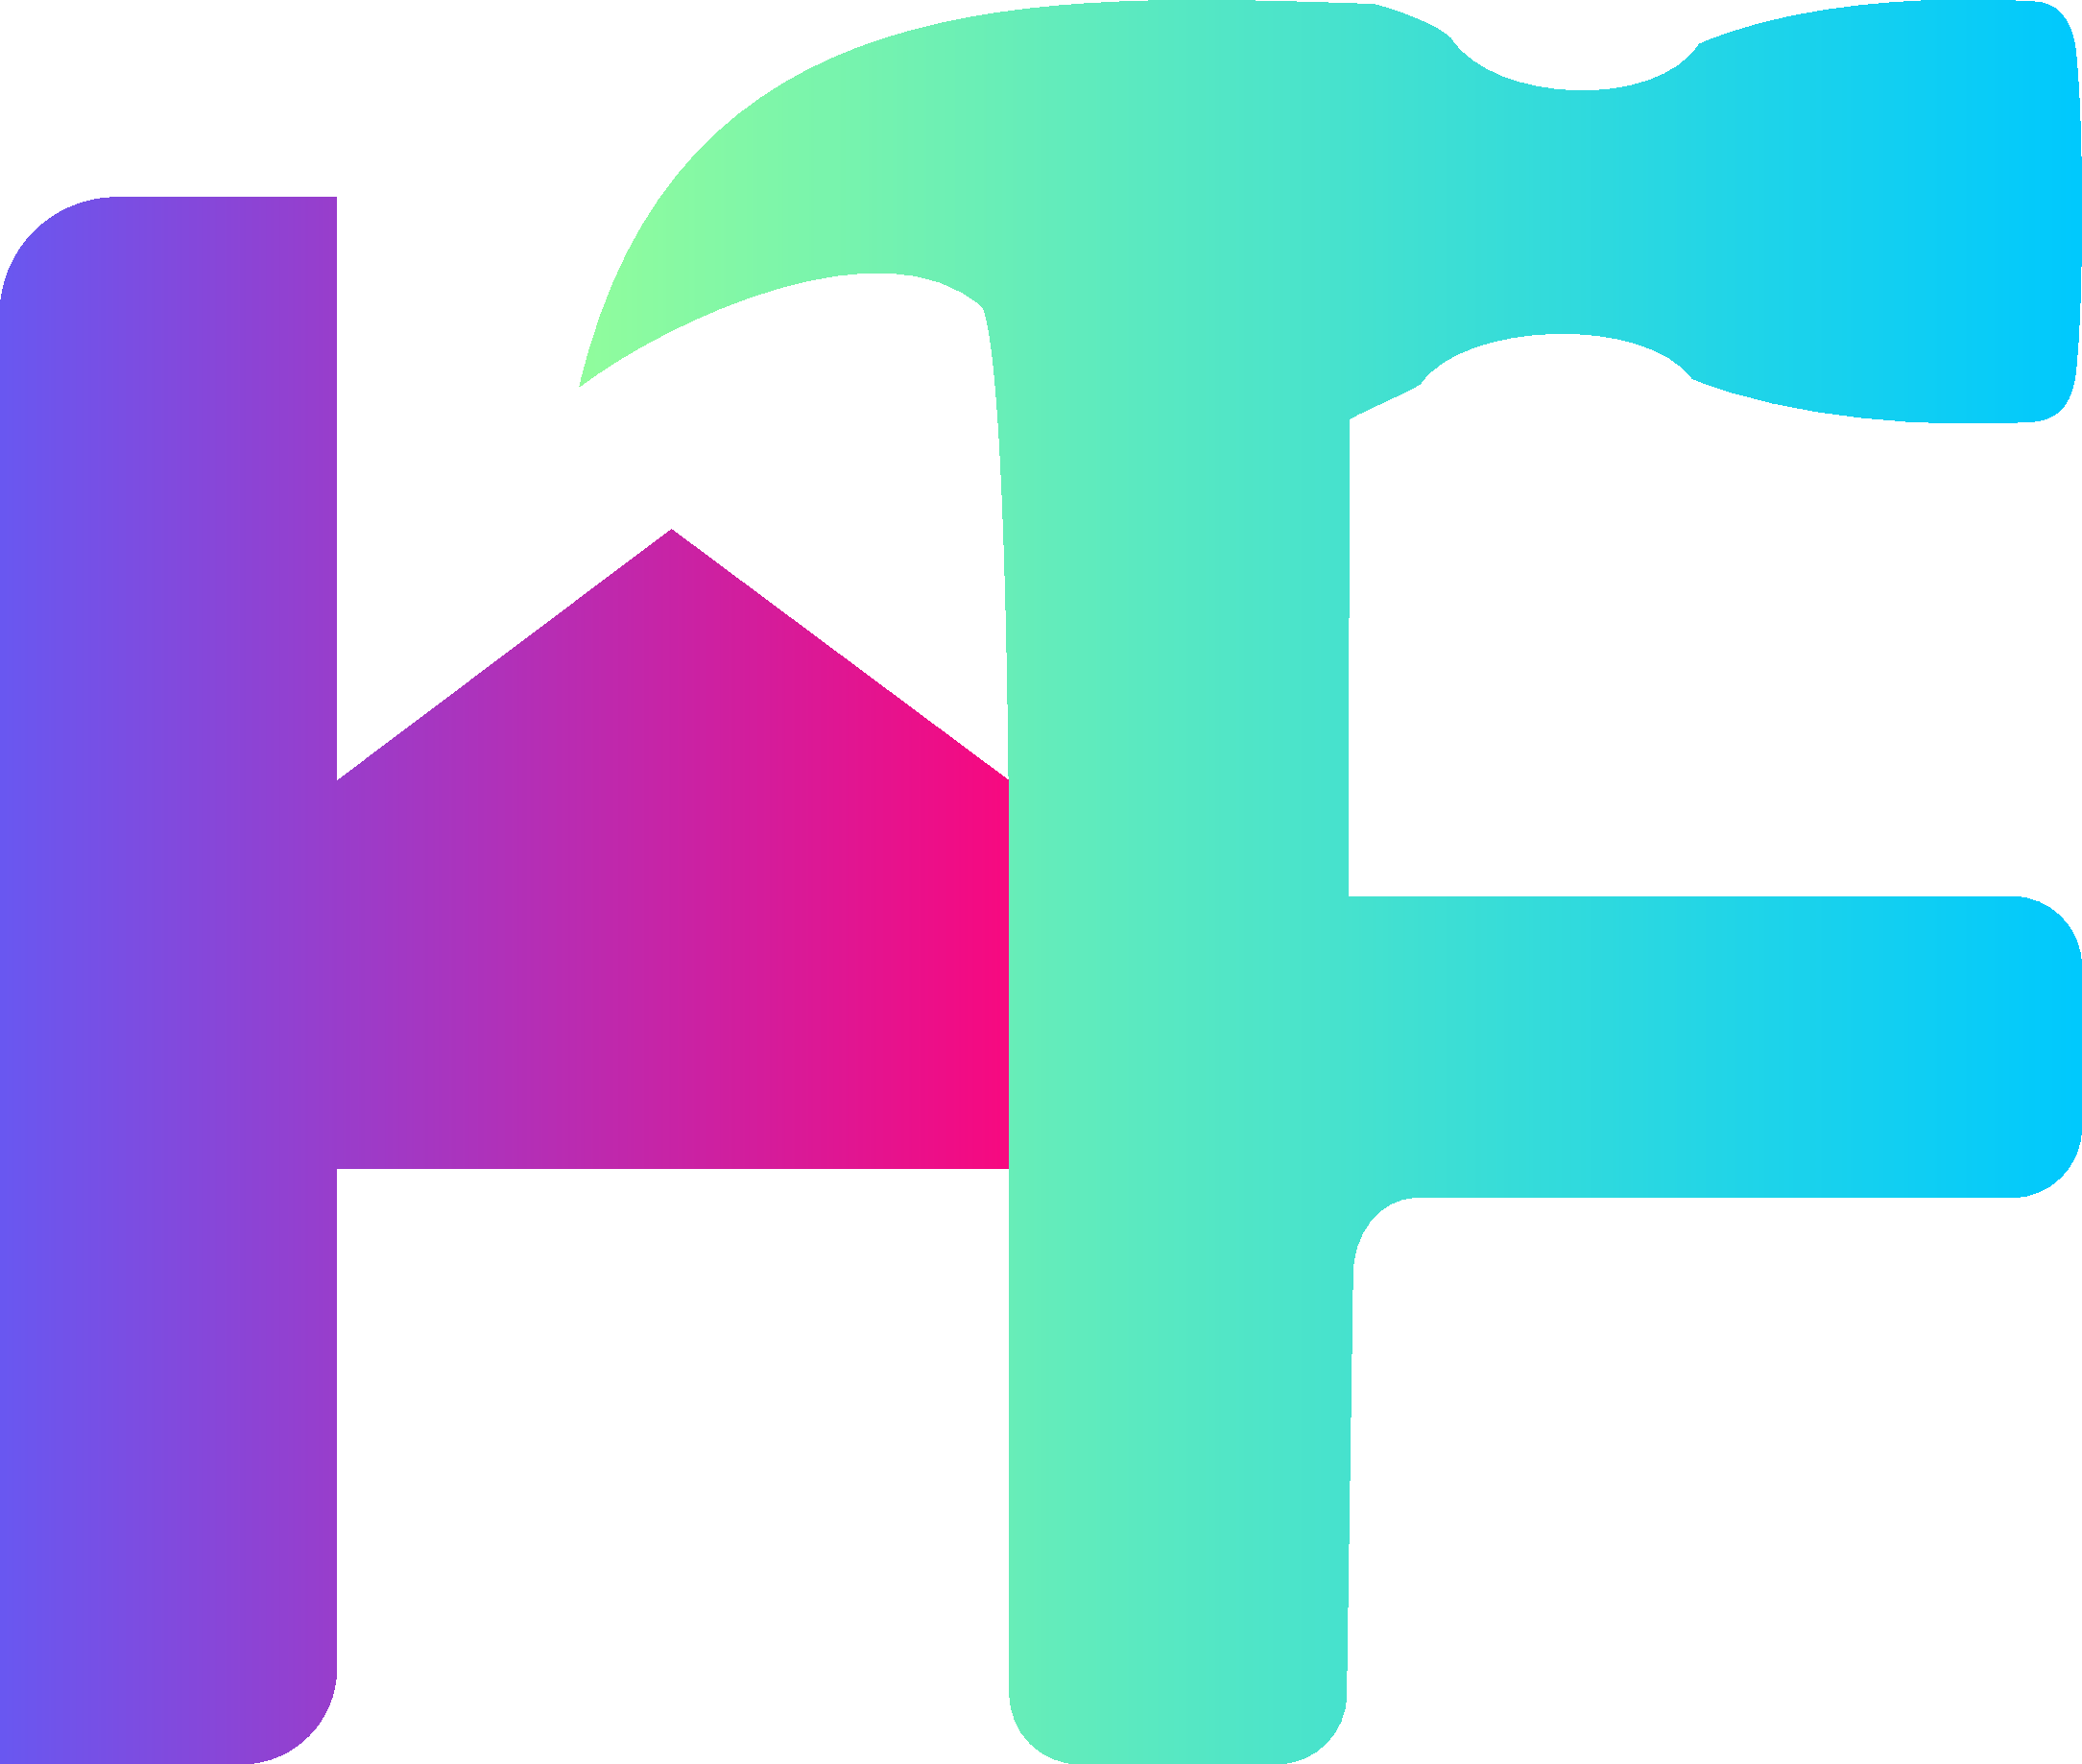
\includegraphics[width=0.4\textwidth]{figuri/HomeForge_v2_color.pdf}
    \caption{Identitatea vizuală a platformei HomeForge}
    \label{fig:homeforge-logo}
\end{figure}

\section{Obiective concrete ale lucrării}
Lucrarea își propune să descrie proiectarea și implementarea HomeForge ca platformă funcțională, urmărind explicit următoarele obiective:

\textbf{Hardware și firmware embedded:}
\begin{itemize}
    \item firmware ESP32 modular care suportă cel puțin patru variante (releu simplu, termostat cu DHT11, termostat cu BMP180, variantă combinată) — vezi directorul \texttt{backend/firmware/projects/};
    \item mecanism de reconectare automată la Wi-Fi și la brokerul MQTT, cu \texttt{ClientID} bazat pe adresa MAC (\textit{watchdog} simplu, fără task-uri FreeRTOS dedicate);
    \item raportare ciclică a stării (\textit{heartbeat}) la fiecare 5 secunde, ascultare continuă pe topicul de comandă.
\end{itemize}

\textbf{Backend Django:}
\begin{itemize}
    \item API REST construit pe Django REST Framework, urmând principiile arhitecturale ale lui Fielding \cite{fielding_rest_dissertation}, cu autentificare JWT \cite{rfc_jwt} și paginare implicită;
    \item daemon MQTT integrat ca \texttt{management command} Django (\texttt{python manage.py mqtt\_listener}), care primește telemetria, o asociază cu device-ul corect prin MAC sau IP și marchează dispozitivele ca \texttt{offline} după 30 de secunde fără heartbeat;
    \item model \texttt{Device} cu o coloană \texttt{JSONField} pentru starea curentă, mapată de Django pe tipul nativ \texttt{JSONB} din PostgreSQL \cite{postgresql_jsonb_docs};
    \item sistem ierarhic de roluri (\texttt{owner}, \texttt{admin}, \texttt{user}) și un mecanism \textit{first-user-becomes-owner} aplicat la înregistrare.
\end{itemize}

\textbf{Frontend Next.js:}
\begin{itemize}
    \item dashboard cu carduri configurabile care suportă \textit{toggle}, \textit{slider} și widget-uri de sensor (temperatură, umiditate, mișcare, lumină, CO\textsubscript{2});
    \item gestionarea layout-ului prin TanStack Query, persistat pe server și cu fallback \texttt{localStorage}, suportând foldere ad-hoc de 2--4 dispozitive în stil iOS;
    \item editor vizual pentru tipuri de dispozitive (\textit{device builder}), cu propunere către administrator, aprobare/respingere și editor de firmware/wiring/documentație;
    \item vizualizare a topologiei rețelei locale folosind React Flow.
\end{itemize}

\textbf{Deployment:}
\begin{itemize}
    \item ambalare în containere Docker pentru backend, frontend și PostgreSQL (vezi \texttt{Dockerfile} și \texttt{Dockerfile});
    \item brokerul Mosquitto rulează în același container cu backend-ul, alături de Avahi pentru discovery mDNS;
    \item script unic de dezvoltare (\texttt{./dev.sh}) care pornește în paralel backend și frontend pentru dezvoltare locală fără Docker.
\end{itemize}

\section{Structura lucrării}
Lucrarea este organizată pe capitole care urmează firul natural de la teorie la implementare:
\begin{itemize}
    \item Capitolul 2 prezintă stadiul actual al tehnologiilor IoT și justifică alegerile făcute (MQTT vs. HTTP, PostgreSQL cu JSONB, stiva Next.js/React).
    \item Capitolul 3 descrie arhitectura backend-ului HomeForge: modelele de date, API-ul REST, autentificarea, daemonul MQTT și mecanismele de aprobare a tipurilor de dispozitive.
    \item Capitolul 4 detaliază aplicația web (Next.js), componentele dashboard-ului, motorul de layout, optimistic UI-ul și editorul vizual de tipuri de dispozitive.
    \item Capitolul 5 acoperă firmware-ul ESP32: protocolul de comunicație, structura proiectelor template și mecanismele de auto-detecție a dispozitivelor.
    \item Capitolul 6 documentează procesul de deployment, containerizarea și pașii de testare manuală.
    \item Capitolul 7 conține concluziile și direcții viitoare de dezvoltare.
\end{itemize}
